\chapter{Result}


\begin{figure}[h]
 \begin{center}
  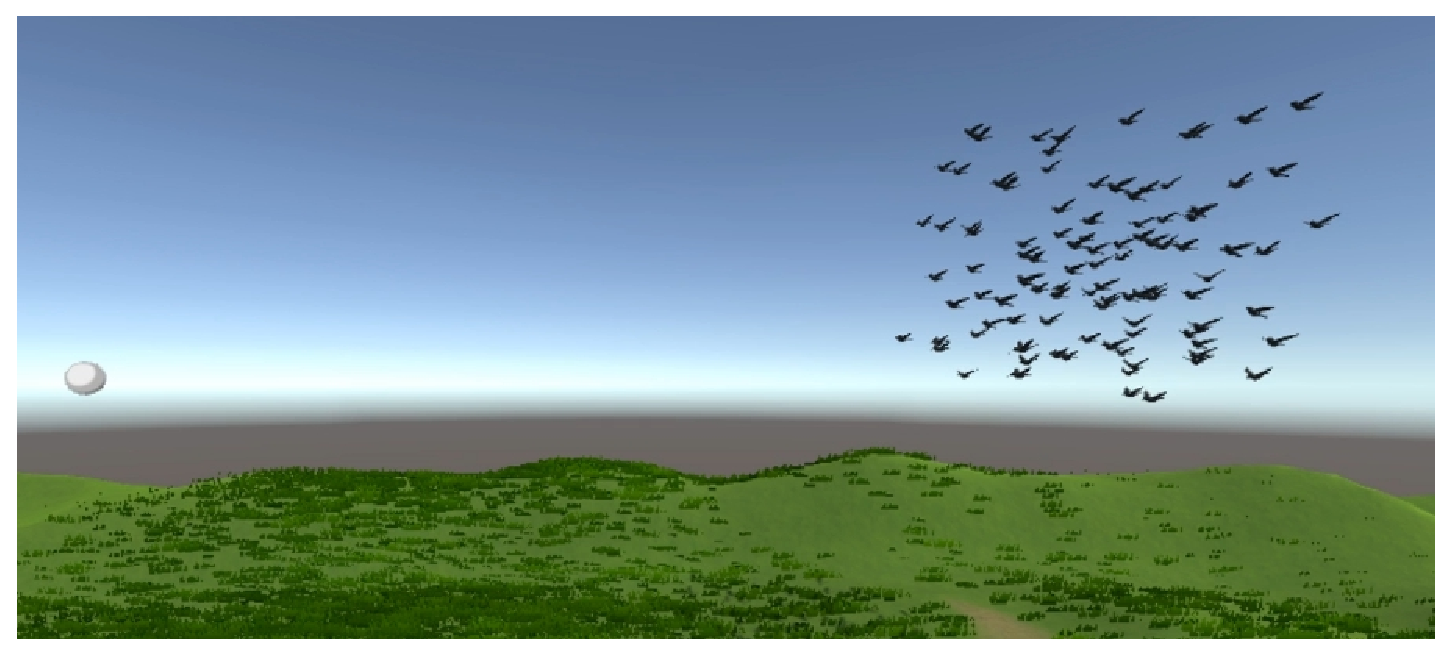
\includegraphics[width=1.0\textwidth]{simulation.eps}
 \end{center}
 \caption{A view of our flock simulation system. The ball on the left is the target for navigating flocks.}
 \label{figure:simulation}
\end{figure}


\section{Flock simulation for generating input video}


For testing our method, a video with bird flock is needed. We planned to use real bird video at first. However, after searching for real bird videos, we found that videos we can find are not good enough as input video, since our approach has several assumptions: all birds stay in the view of camera, camera is not moving, and 


Due to difficulties mentioned above, we implemented a bird flock simulation system and capture the flock motion as input video to test our method. The simulation system is based on boid model, which assumes a flock is simply the result of the interaction between the behaviors of individual birds. With these behaviors, the system can produce fine flock motion with numbers of birds. However, boid model can only model flock wandering behavior. That is, after assigning initial parameters, all birds become uncontrollable during the simulation, and the simulation always produces same results. To keep the diversity of the generated simulation result, we further include the homing behavior introduced in \cite{Shape,OB1}. With this behavior, we can generate different flock motions efficiently. After the simulation result is generated, we capture videos from a view, the captured video is then used as input video to the system. Figure \ref{figure:simulation} shows a view of our flock simulation system.


\section{Generated flock motion}


We have used 3 input videos to test our system. The first one is a real bird video taken by ourselves, while the other two are generated input videos from our flock simulation system.  Information and parameters of three input videos are shown in Table \ref{table:result}.


\begin{table}[h]
\begin{tabular}{|l|l|l|l|l|l|l|l|l|}
\hline
  & resolution & \# of birds & \# of frames & $v_{target}$ & $\lambda_{t}$ & $\lambda_{f}$ & $w_{sep}$ & $d_{sep}$ \\ \hline
Result 1 (real video) & 854x480    & 4           & 120          & 0.1          & 0.3           & 1.0           & 2         & 0.9       \\ \hline
Result 2 (united)     & 1280x720   & 10          &              &              &               &               &           &           \\ \hline
Result 3 (separated)  & 1280x720   & 5           & 230          & 0.5          & 0.3           & 0.1           & 2         & 0.8       \\ \hline
\end{tabular}
\caption{Information and optimization parameters of 3 input videos.}
\label{table:result}
\end{table}


%\begin{figure}[h]
% \begin{center}
%  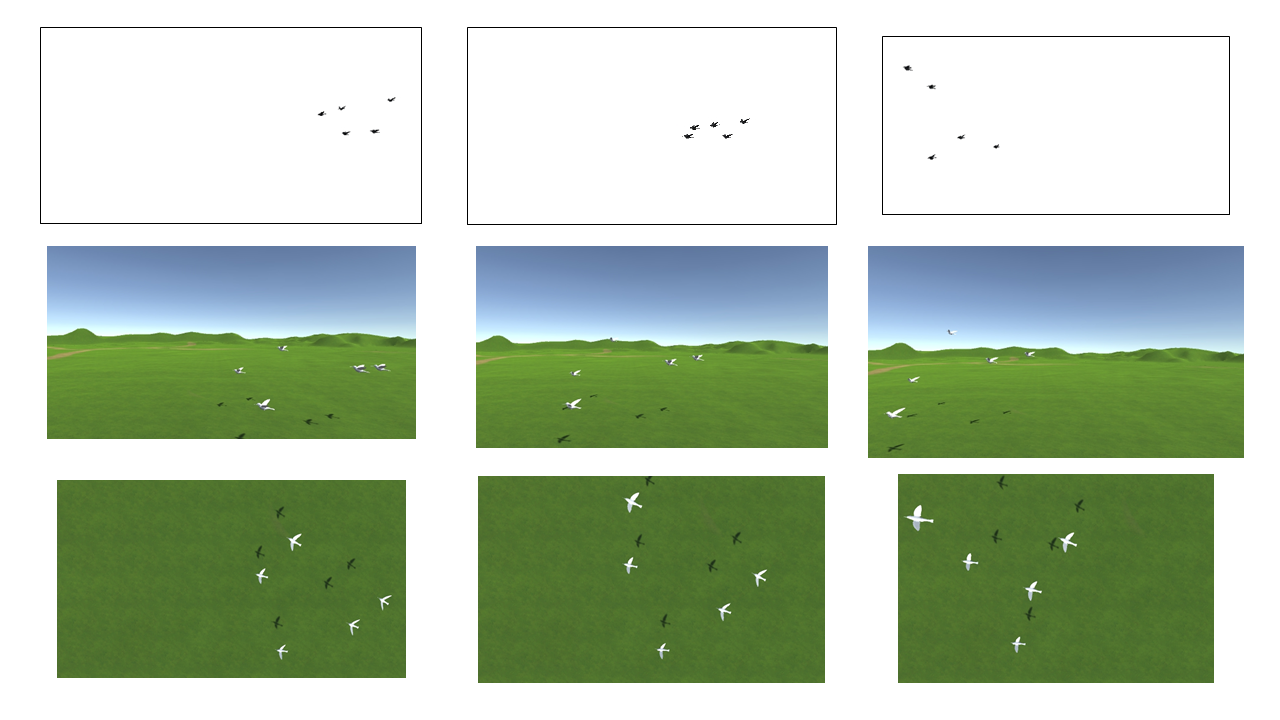
\includegraphics[width=1.0\textwidth]{result1.eps}
% \end{center}
% \caption{Result1:(top)input video. (middle)generated result from side view. (bottom)generated result from top view.}
% \label{figure:result1_side}
%\end{figure}


Figure \ref{figure:result1_com} shows our first result from real bird video. The video is relatively short and has less birds, and camera also  slightly moves when recording. Although the quality of the input video is not good. we test our system first with this real video before using generated video as input. Results of 3 frames in sequence are shown in Figure \ref{figure:result1_com}. The first row is the input video, and the second, third rows are generated flock motions in camera view and top view.



\begin{figure}[h]
\begin{center}
\subfloat[Input video]{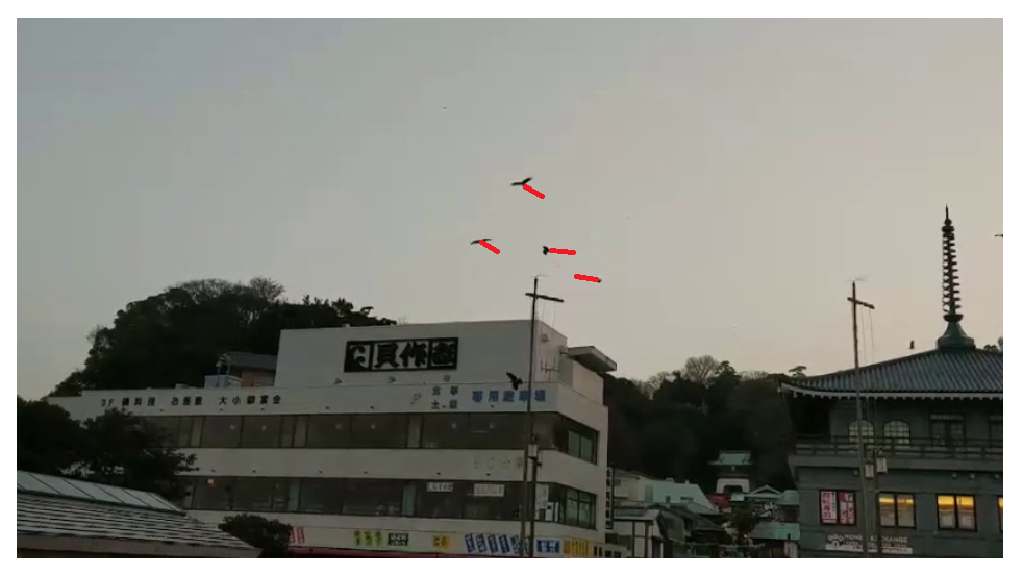
\includegraphics[width=.3\textwidth]{result_1_input_40.eps}}\hspace{\fill}
\subfloat[]{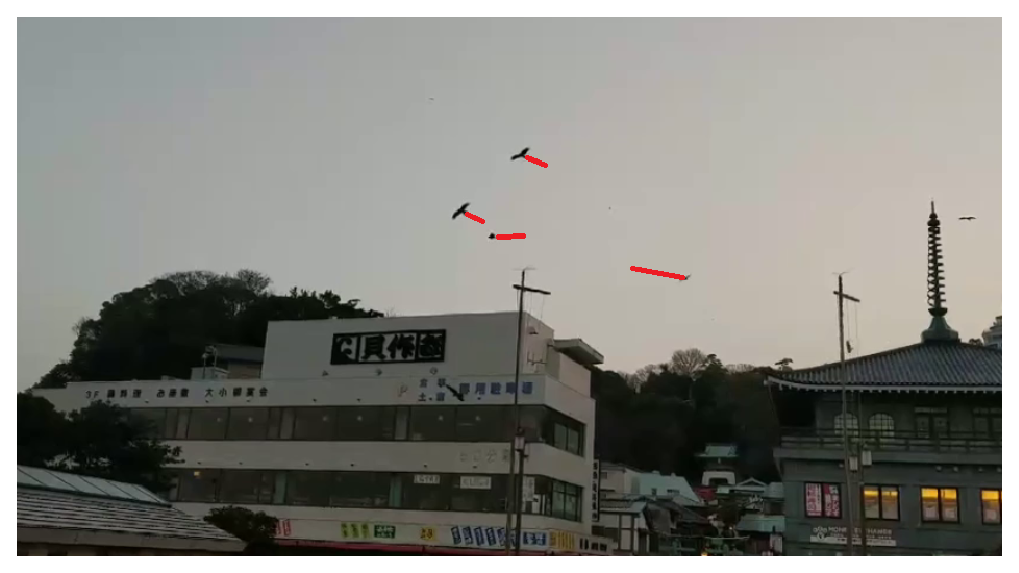
\includegraphics[width=.3\textwidth]{result_1_input_60.eps}}\hspace{\fill}
\subfloat[]{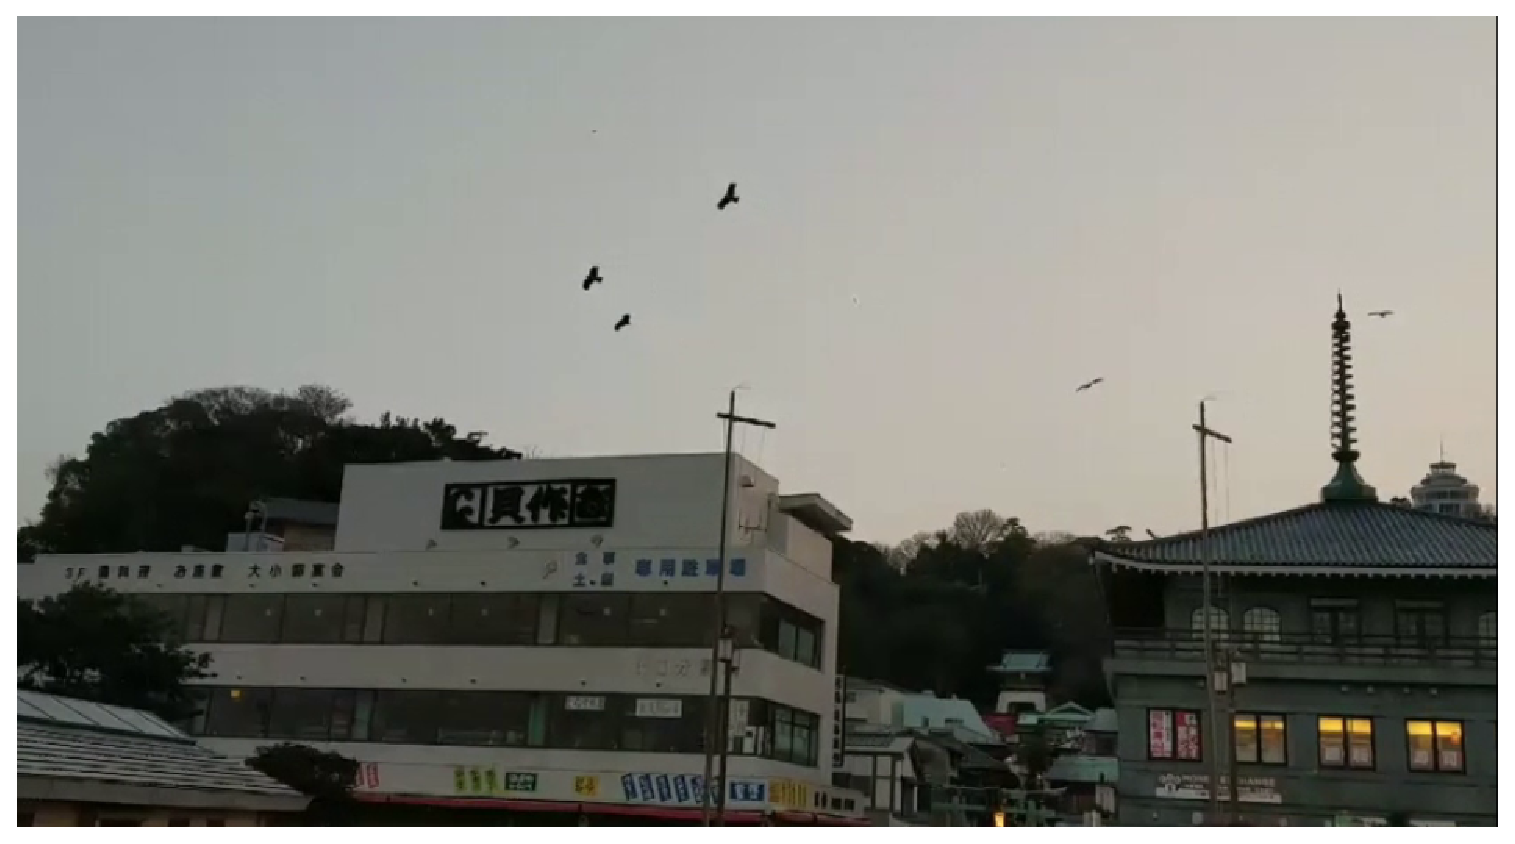
\includegraphics[width=.3\textwidth]{result_1_input_80.eps}}


\subfloat[Result (camera view)]{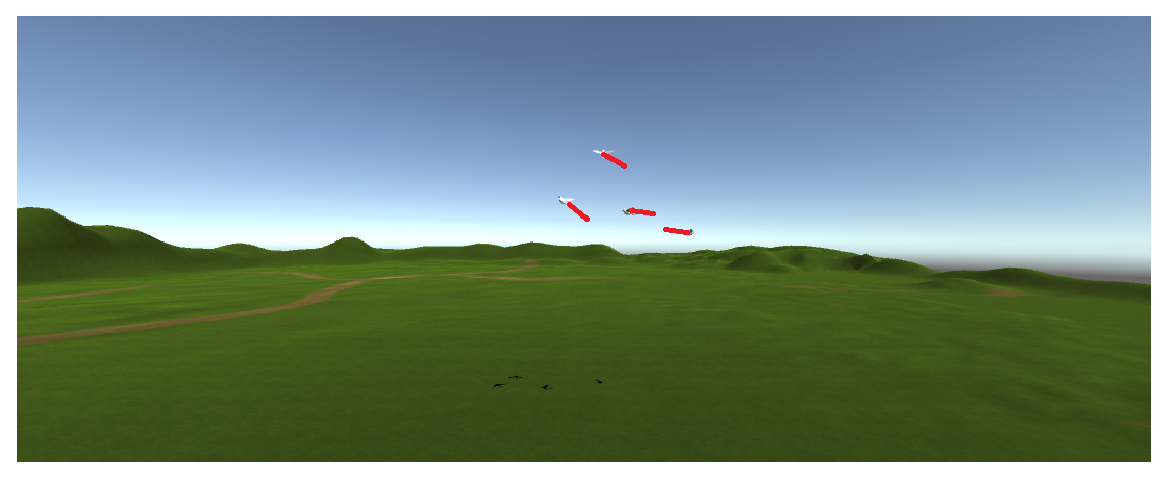
\includegraphics[width=.3\textwidth]{result_1_side_40.eps}}\hspace{\fill}
\subfloat[]{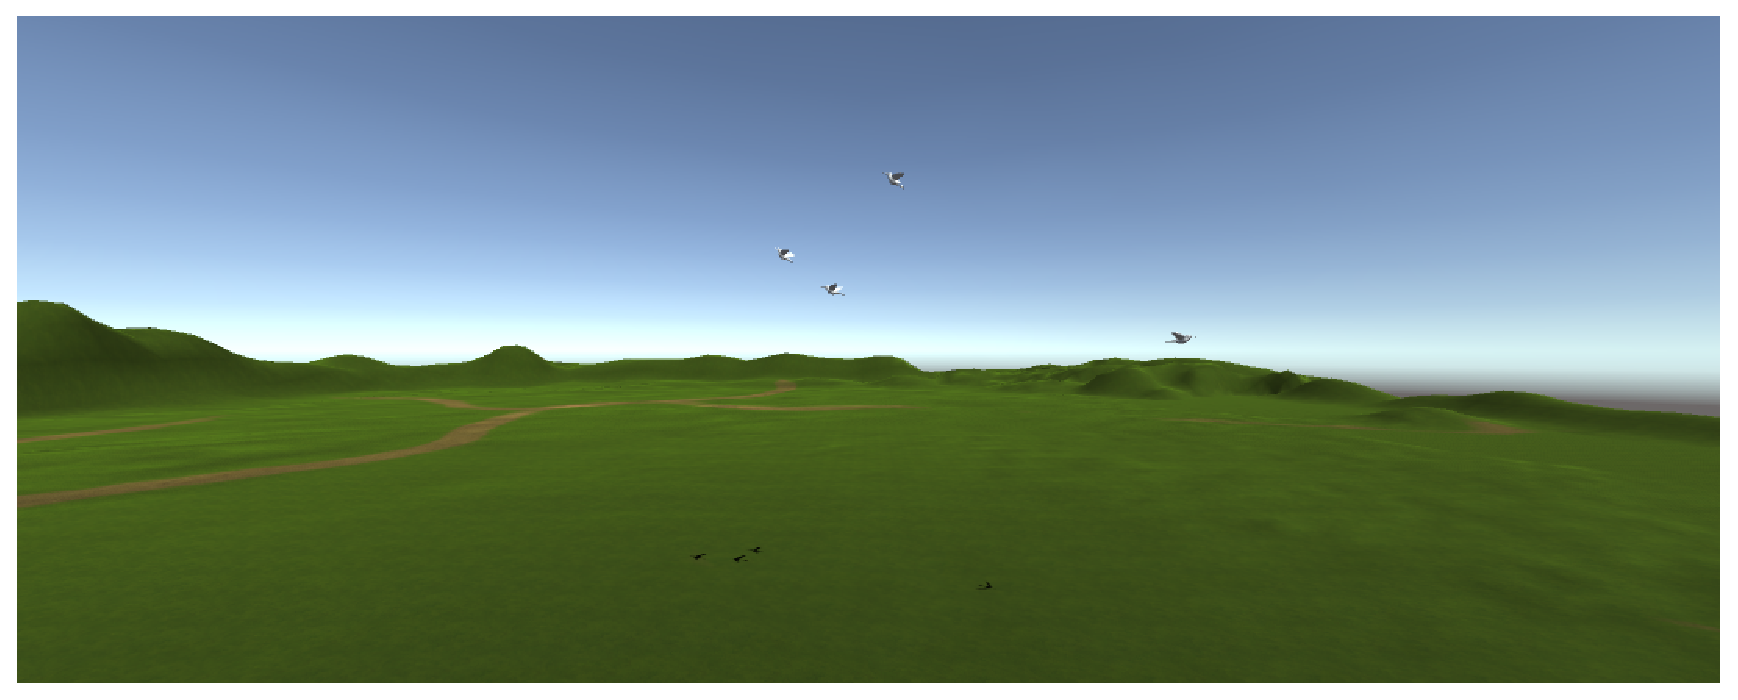
\includegraphics[width=.3\textwidth]{result_1_side_60.eps}}\hspace{\fill}
\subfloat[]{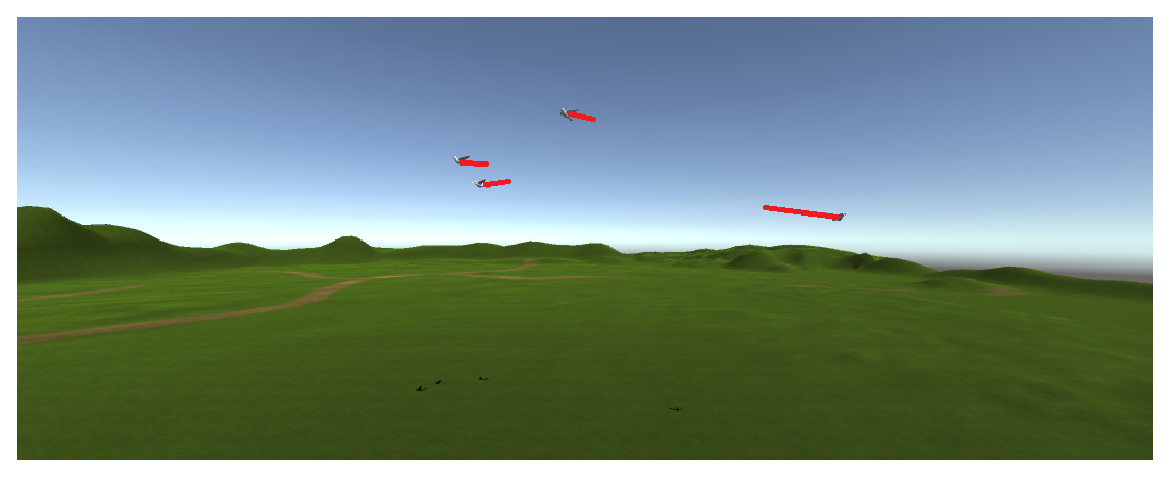
\includegraphics[width=.3\textwidth]{result_1_side_80.eps}}


\subfloat[Result (top view)]{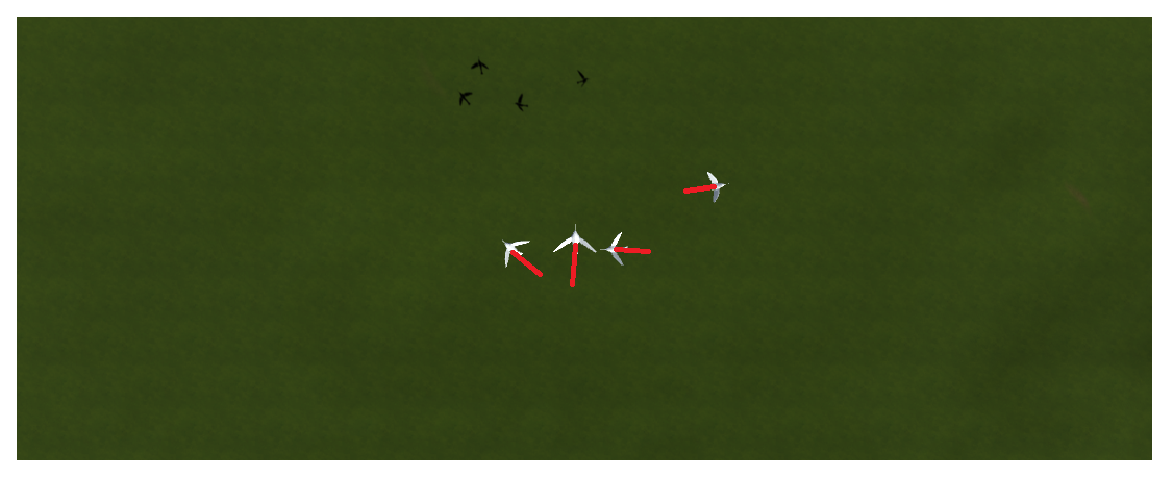
\includegraphics[width=.3\textwidth]{result_1_top_40.eps}}\hspace{\fill}
\subfloat[]{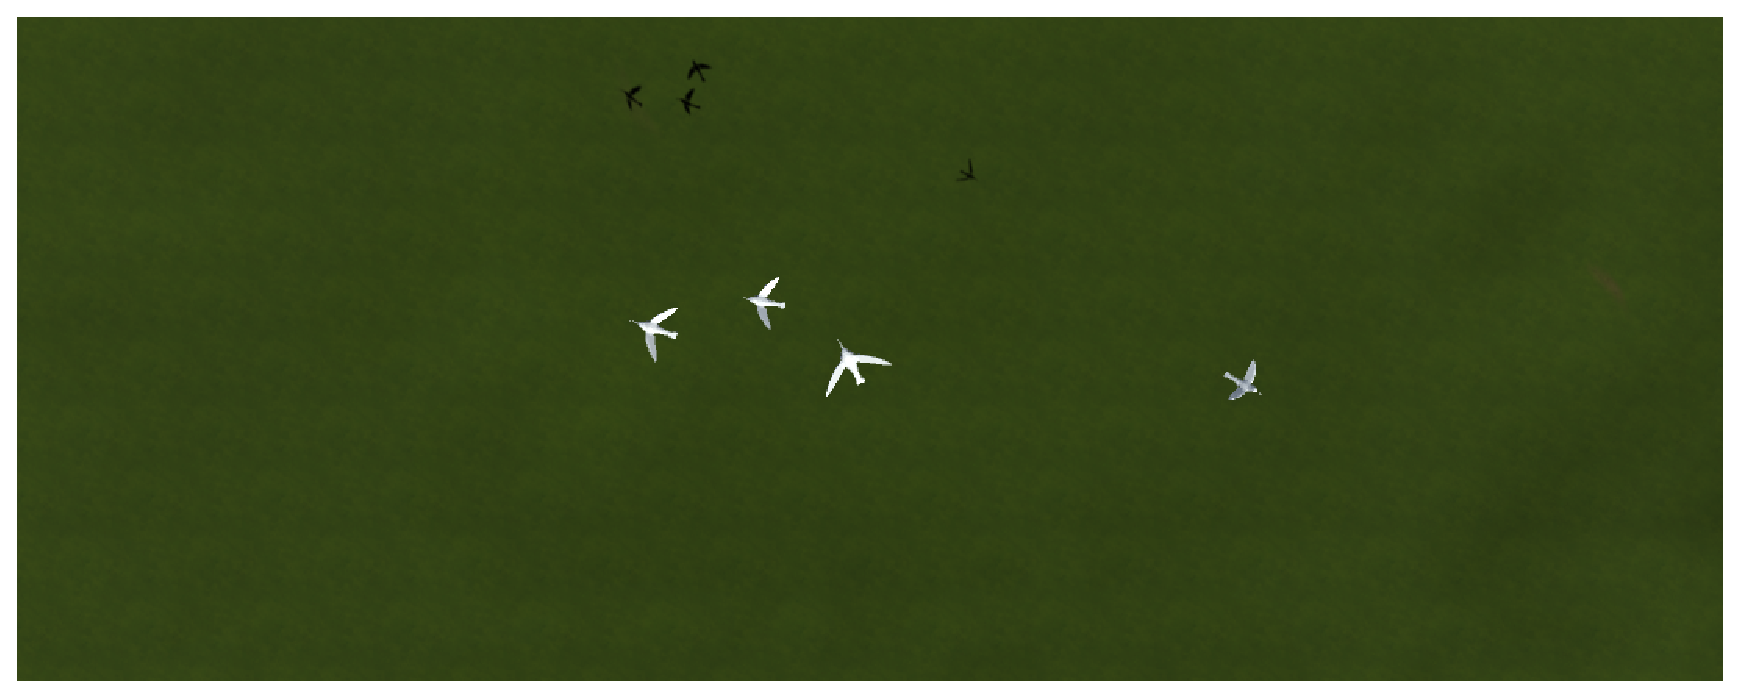
\includegraphics[width=.3\textwidth]{result_1_top_60.eps}}\hspace{\fill}
\subfloat[]{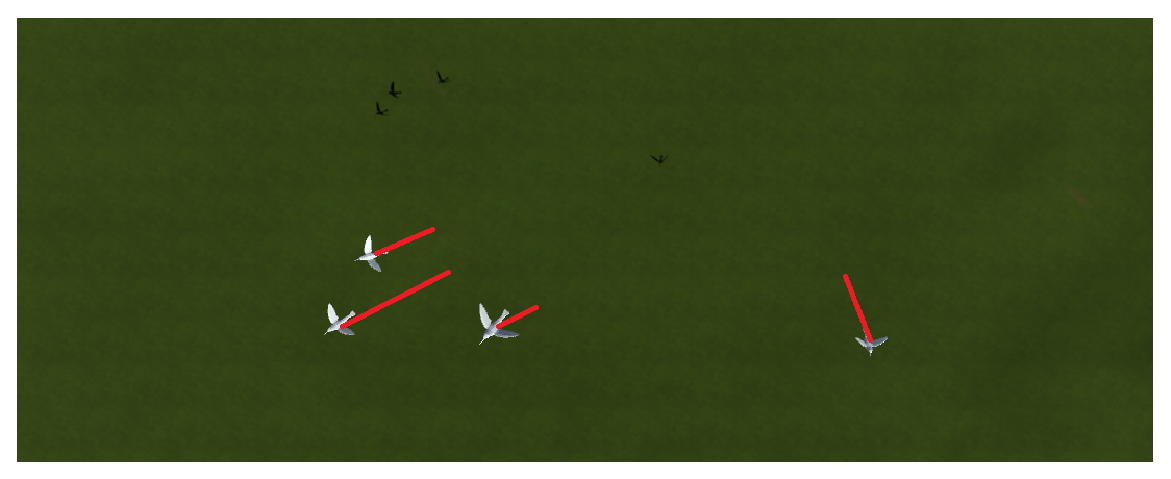
\includegraphics[width=.3\textwidth]{result_1_top_80.eps}}
\end{center}
\caption{Comparison of Result 1 in frame 40, 60, 80.}
\label{figure:result1_com}
\end{figure}


However, since result 1 is too short and lack of numbers to observe flock behavior, we use generated video instead for testing various conditions. Based on our observation on bird flocks, we think that bird flock can be categorized into two types: united flock and separate flock, depending on the relativity between birds in a flock. Thus, we decide to make two kinds of bird flocks to test if the system is capable of having these two kinds of flock motion.


Figure \ref{figure:result2_com1} and Figure \ref{figure:result2_com2} show our results from video generated by our flock simulation system. The video is relatively long and has 10 birds flying around an object. In this video, bird flock flies in a united form. Birds fly in similar direction during the whole video. This video is used to evaluate the ability of united flocks. In the generated flock motion, flock behavior can be observed: birds stay united and collision avoidance is well done. Turning happens in frame 80 and 100, and the generated motion also turns smoothly, based on trajectory smoothness term in optimization algorithm.


\begin{figure}[p]
\begin{center}
\subfloat[Input video]{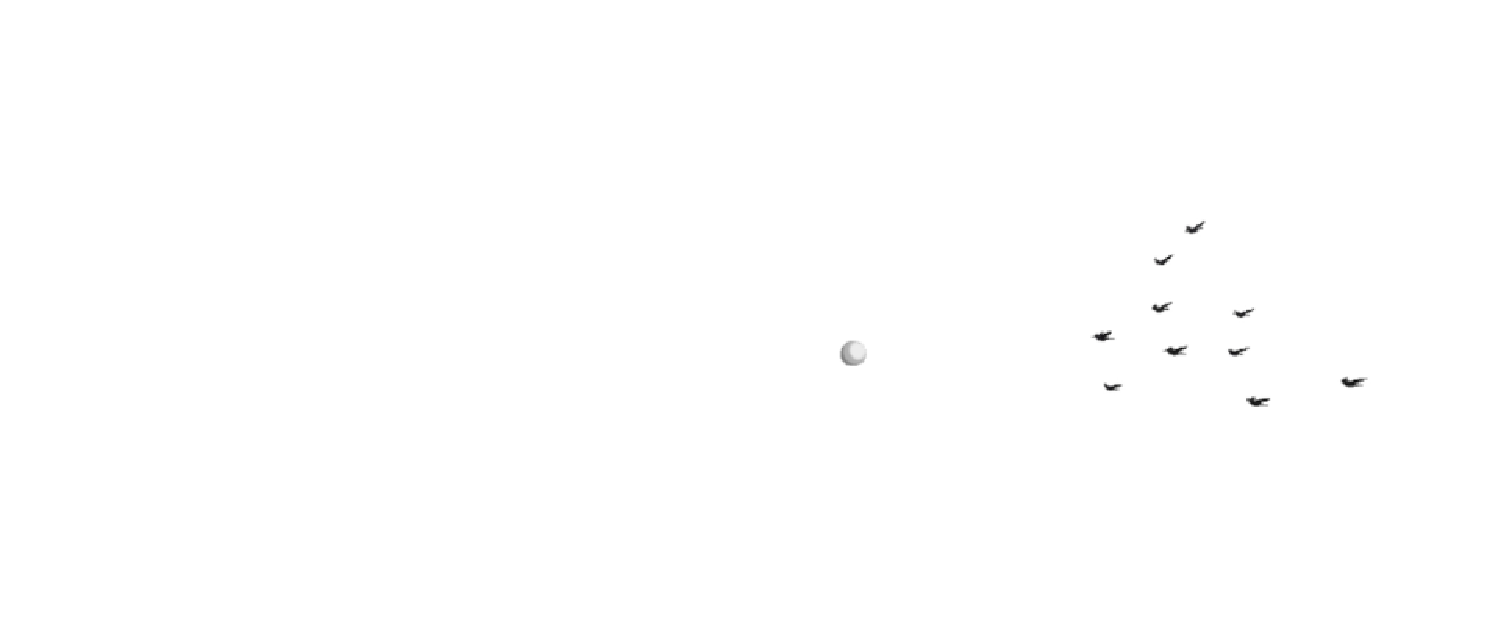
\includegraphics[width=.3\textwidth]{result_2_input_0.eps}}\hspace{\fill}
\subfloat[]{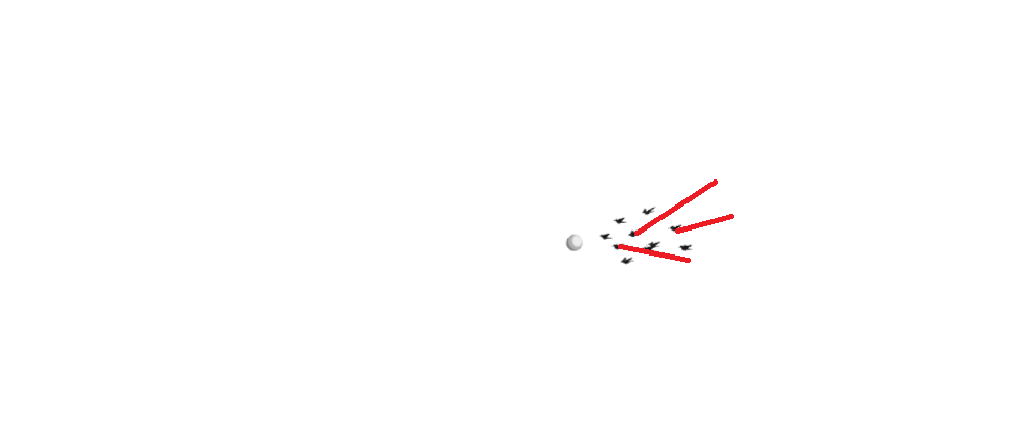
\includegraphics[width=.3\textwidth]{result_2_input_20.eps}}\hspace{\fill}
\subfloat[]{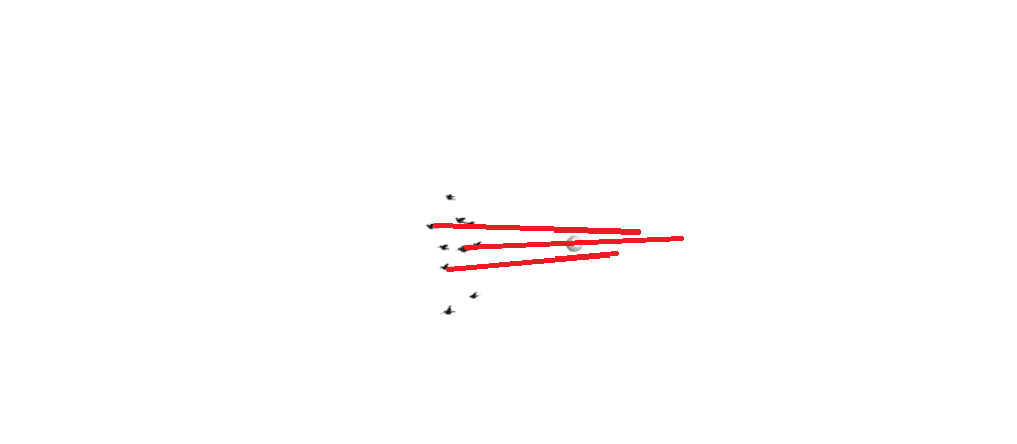
\includegraphics[width=.3\textwidth]{result_2_input_40.eps}}


\subfloat[Result (camera view)]{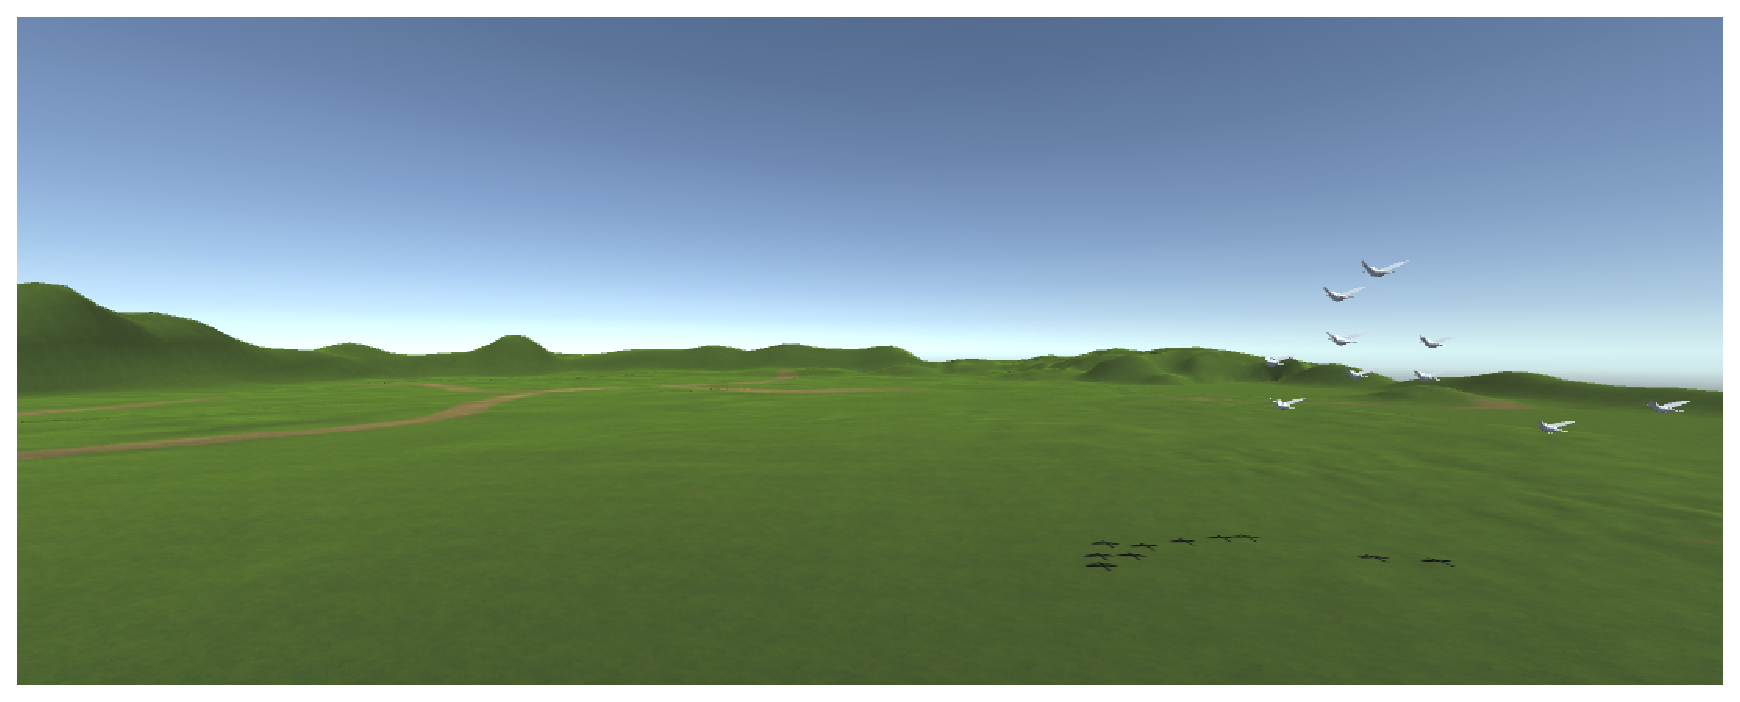
\includegraphics[width=.3\textwidth]{result_2_side_0.eps}}\hspace{\fill}
\subfloat[]{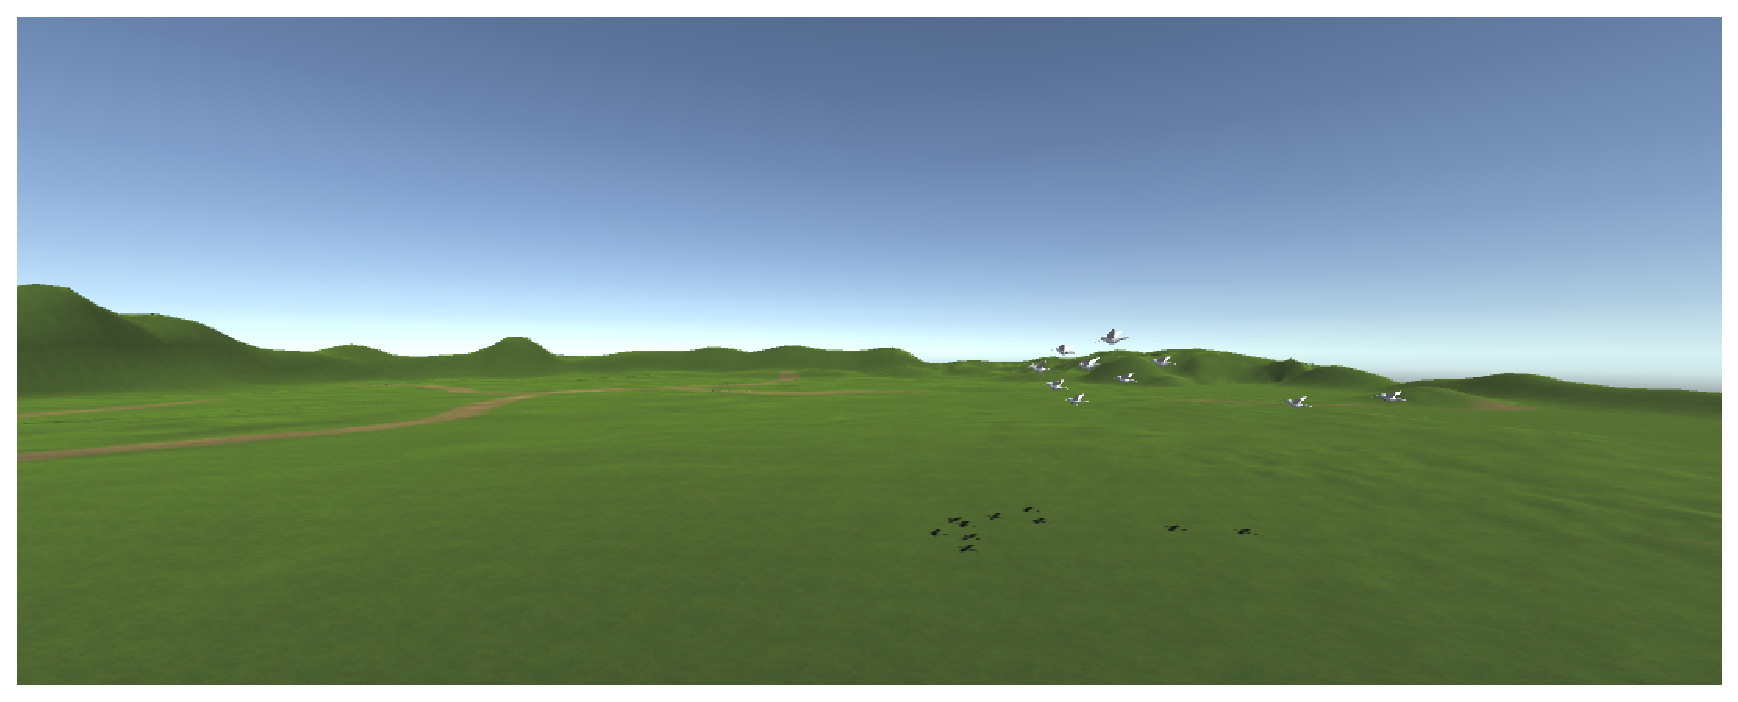
\includegraphics[width=.3\textwidth]{result_2_side_20.eps}}\hspace{\fill}
\subfloat[]{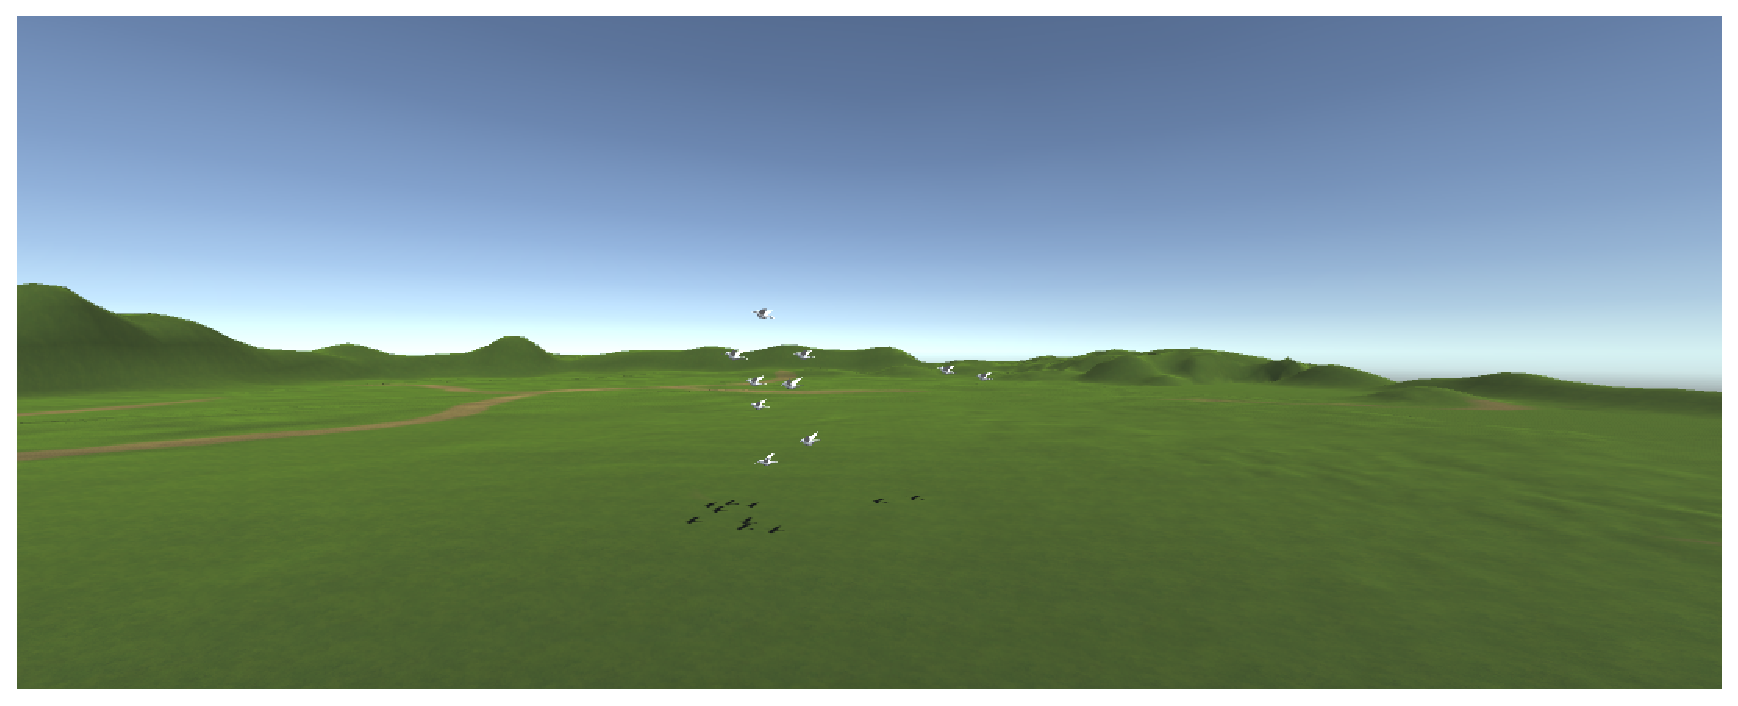
\includegraphics[width=.3\textwidth]{result_2_side_40.eps}}


\subfloat[Result (top view)]{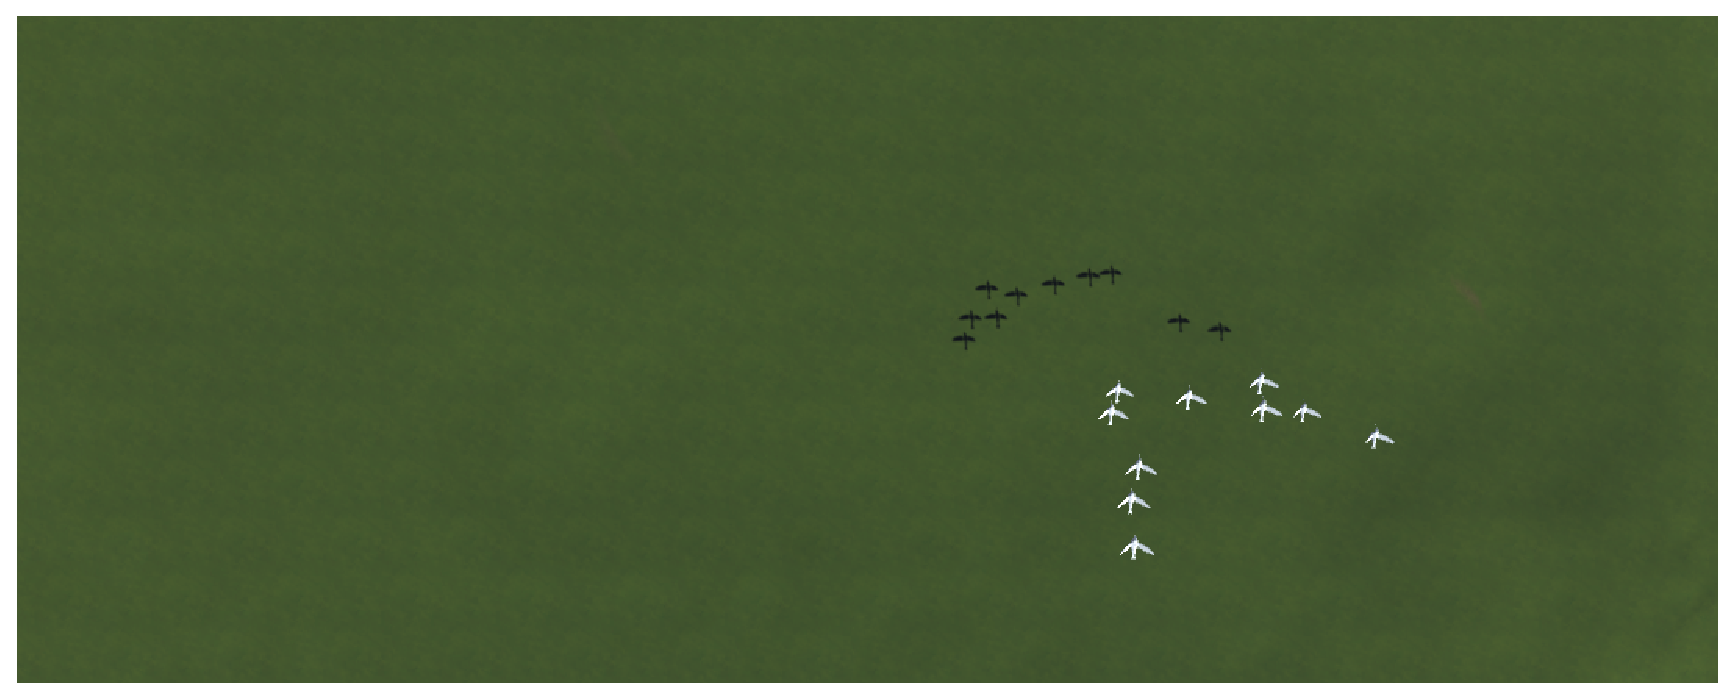
\includegraphics[width=.3\textwidth]{result_2_top_0.eps}}\hspace{\fill}
\subfloat[]{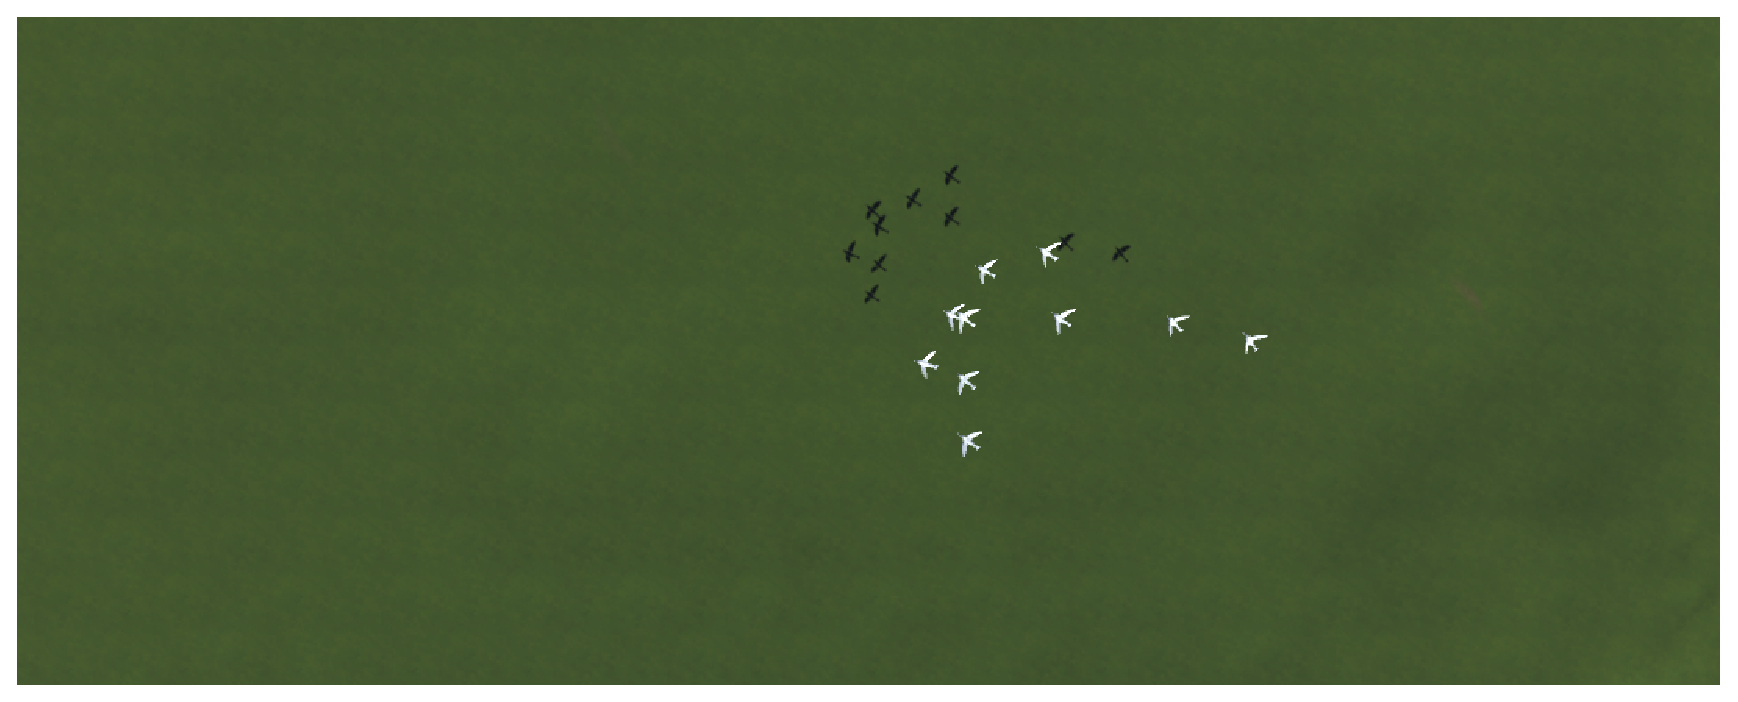
\includegraphics[width=.3\textwidth]{result_2_top_20.eps}}\hspace{\fill}
\subfloat[]{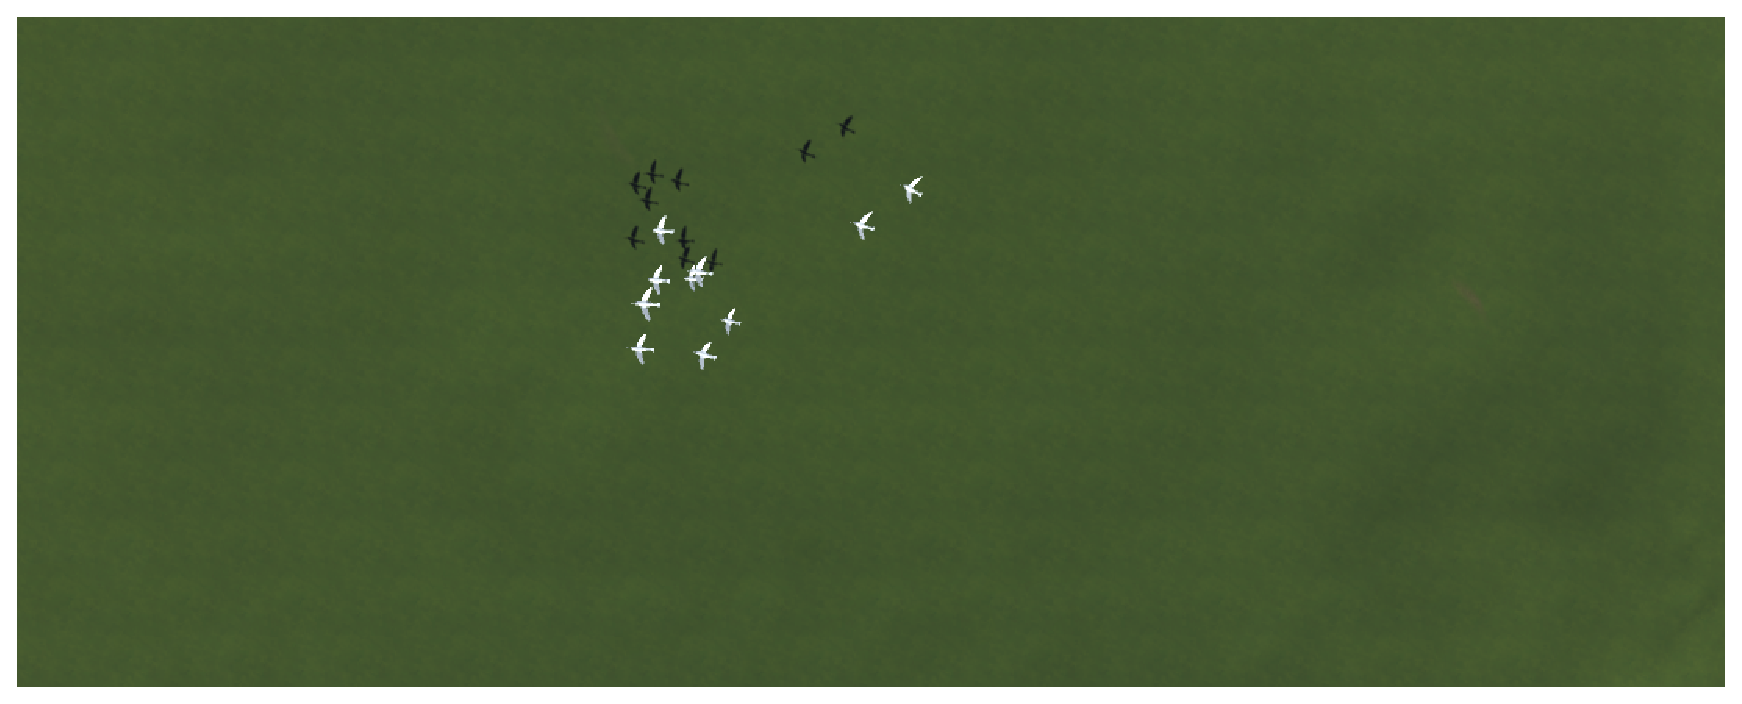
\includegraphics[width=.3\textwidth]{result_2_top_40.eps}}
\end{center}
\caption{Comparison of Result 2 in frame 0, 20, 40.}
\label{figure:result2_com1}
\end{figure}


\begin{figure}[p]
\begin{center}
\subfloat[Input video]{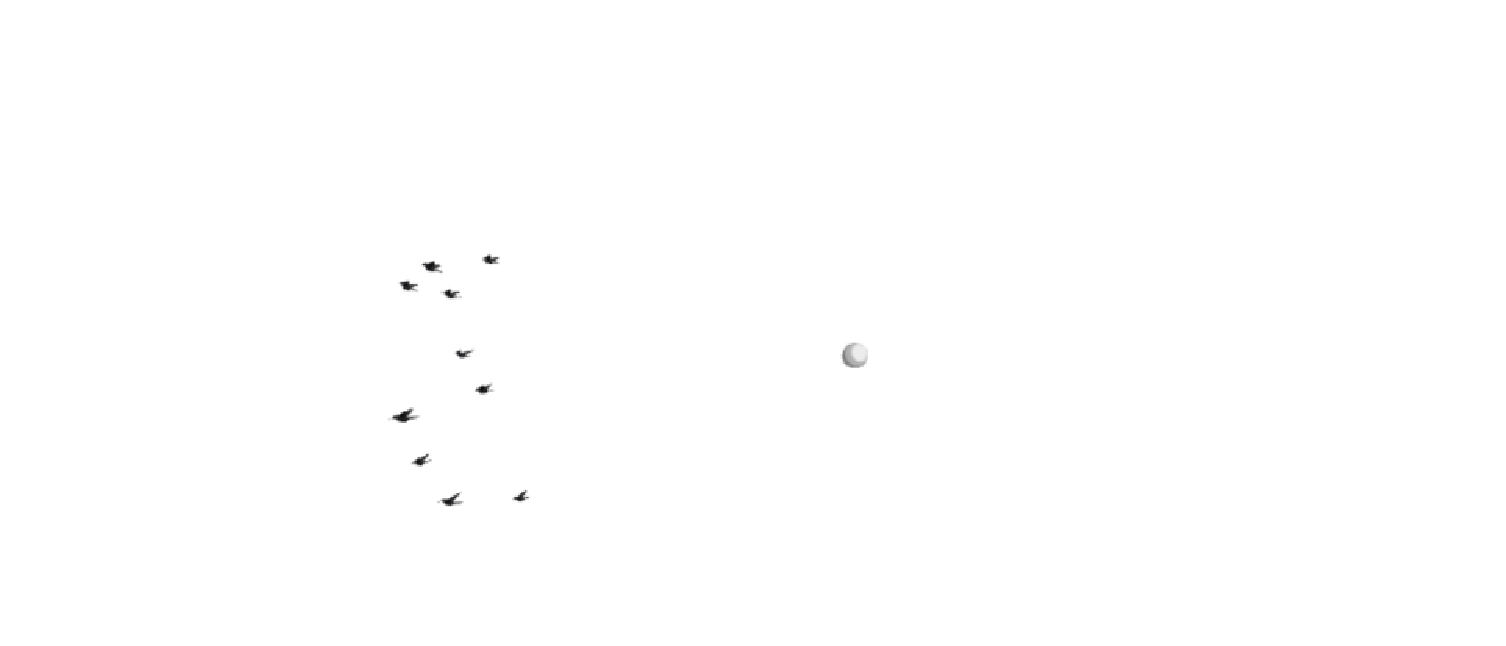
\includegraphics[width=.3\textwidth]{result_2_input_60.eps}}\hspace{\fill}
\subfloat[]{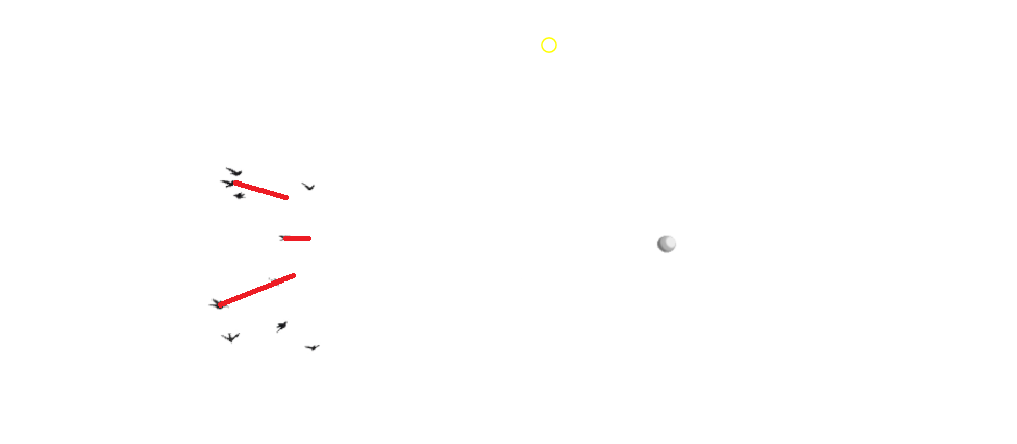
\includegraphics[width=.3\textwidth]{result_2_input_80.eps}}\hspace{\fill}
\subfloat[]{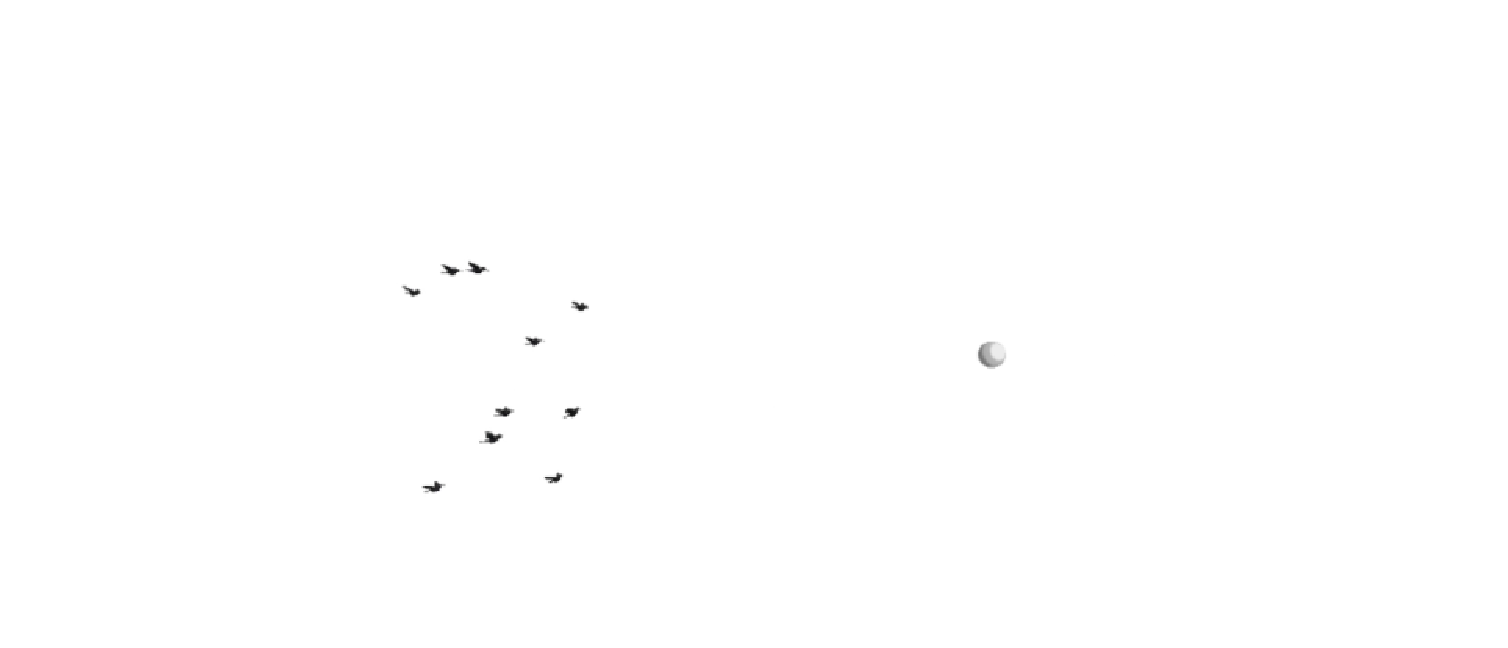
\includegraphics[width=.3\textwidth]{result_2_input_100.eps}}


\subfloat[Result (camera view)]{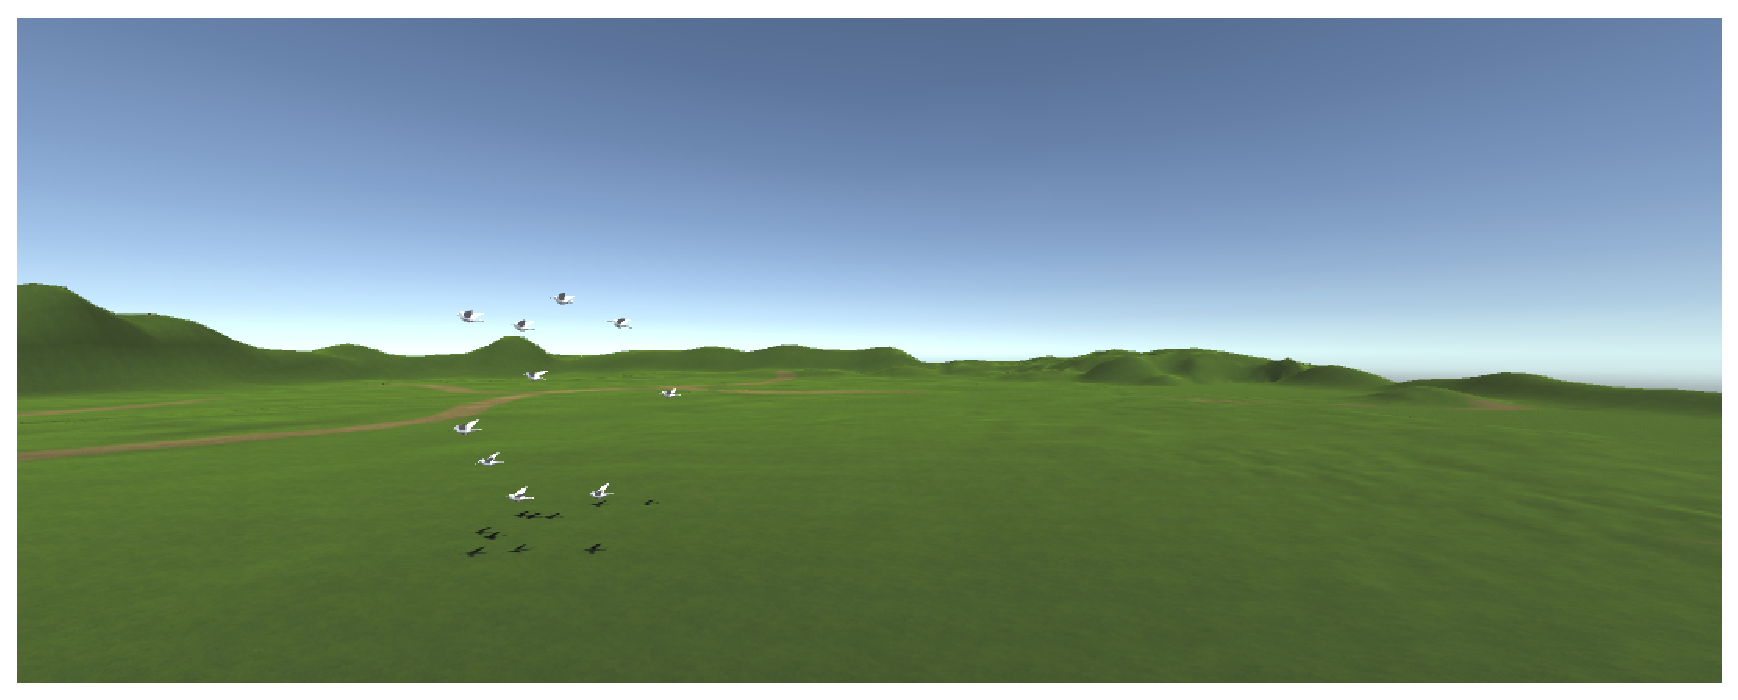
\includegraphics[width=.3\textwidth]{result_2_side_60.eps}}\hspace{\fill}
\subfloat[]{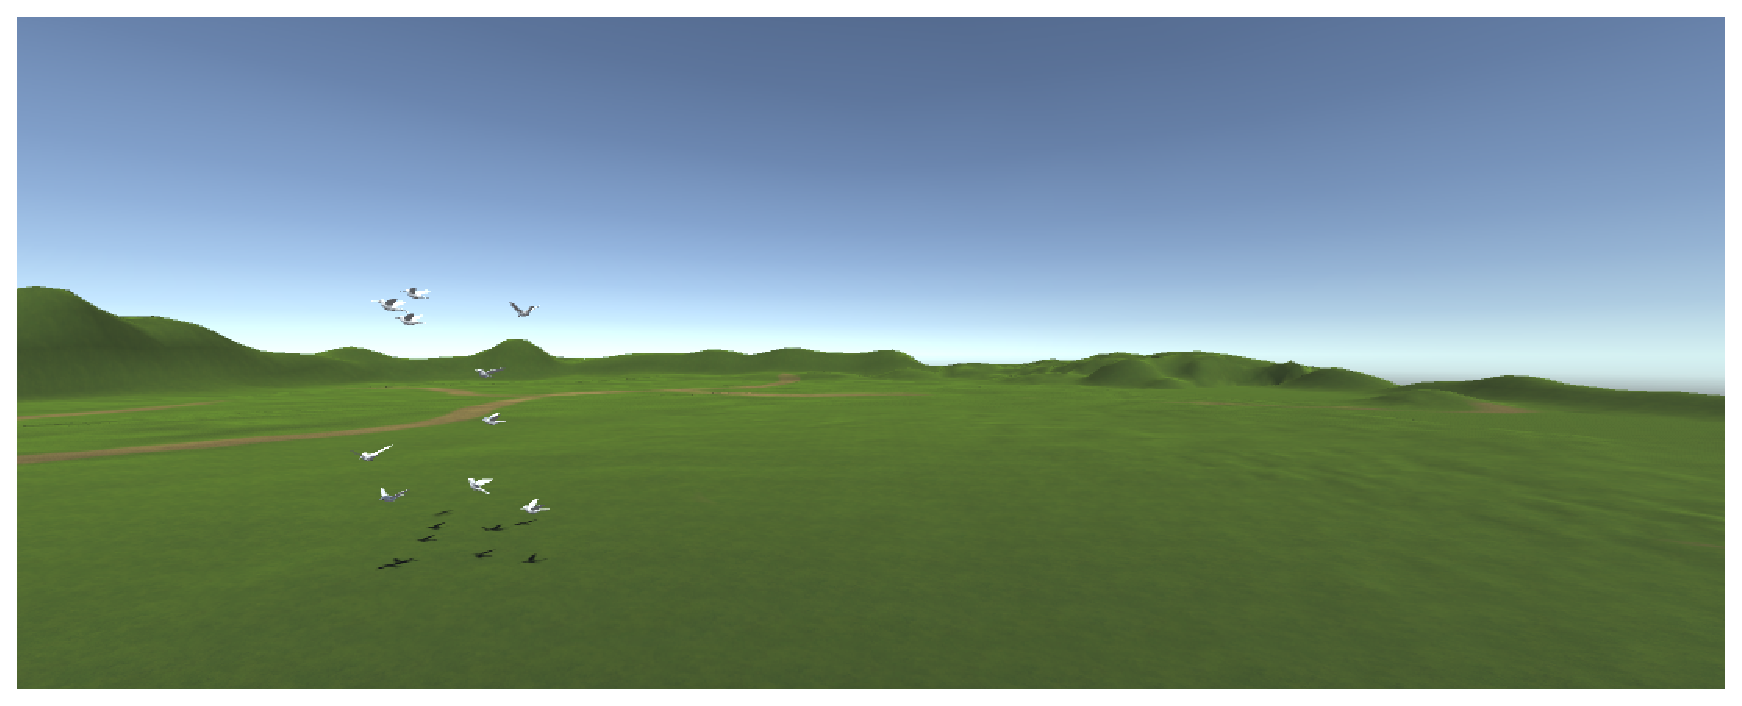
\includegraphics[width=.3\textwidth]{result_2_side_80.eps}}\hspace{\fill}
\subfloat[]{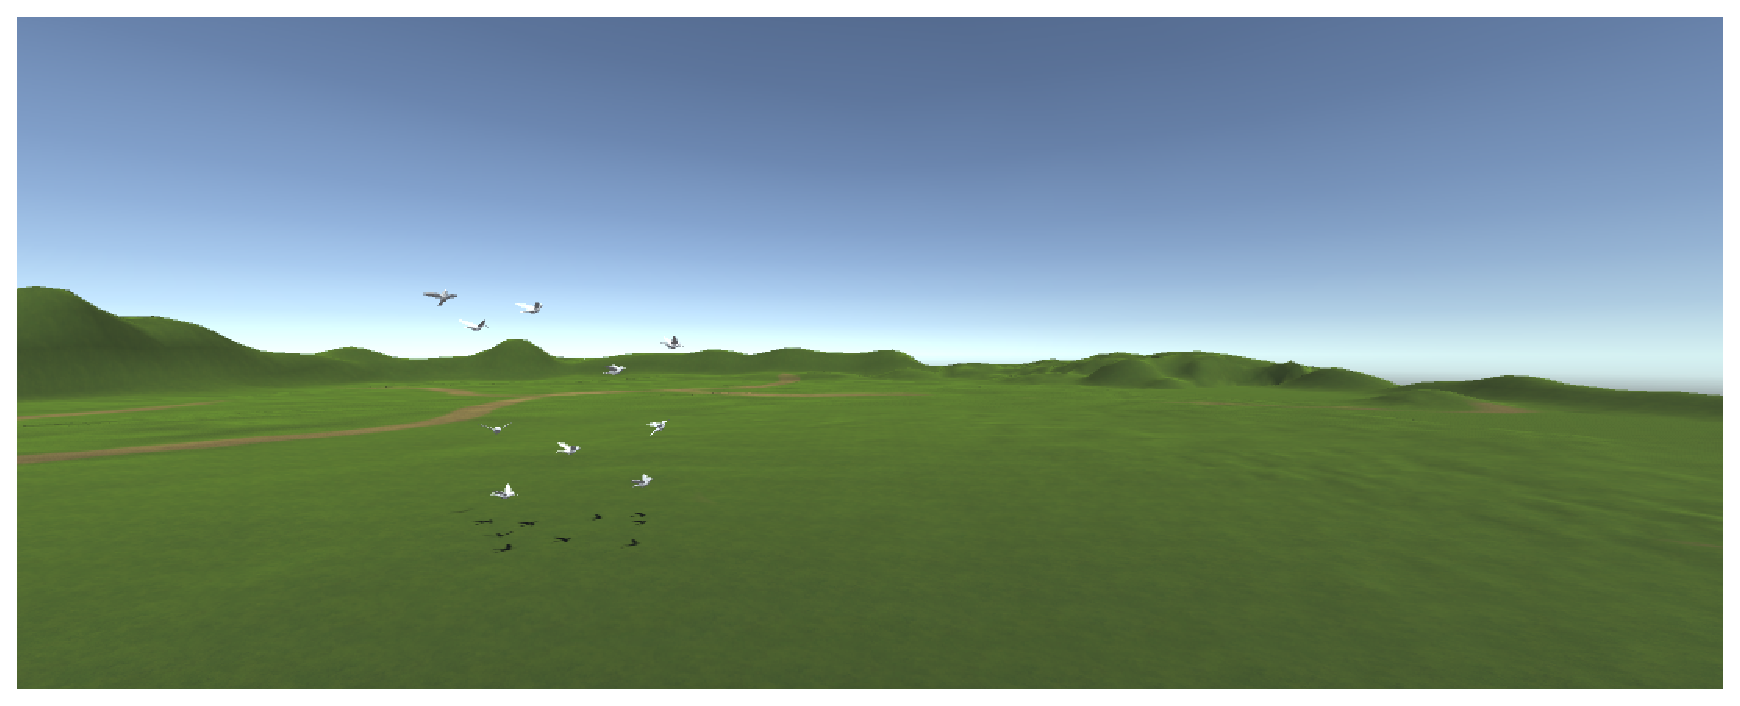
\includegraphics[width=.3\textwidth]{result_2_side_100.eps}}


\subfloat[Result (top view)]{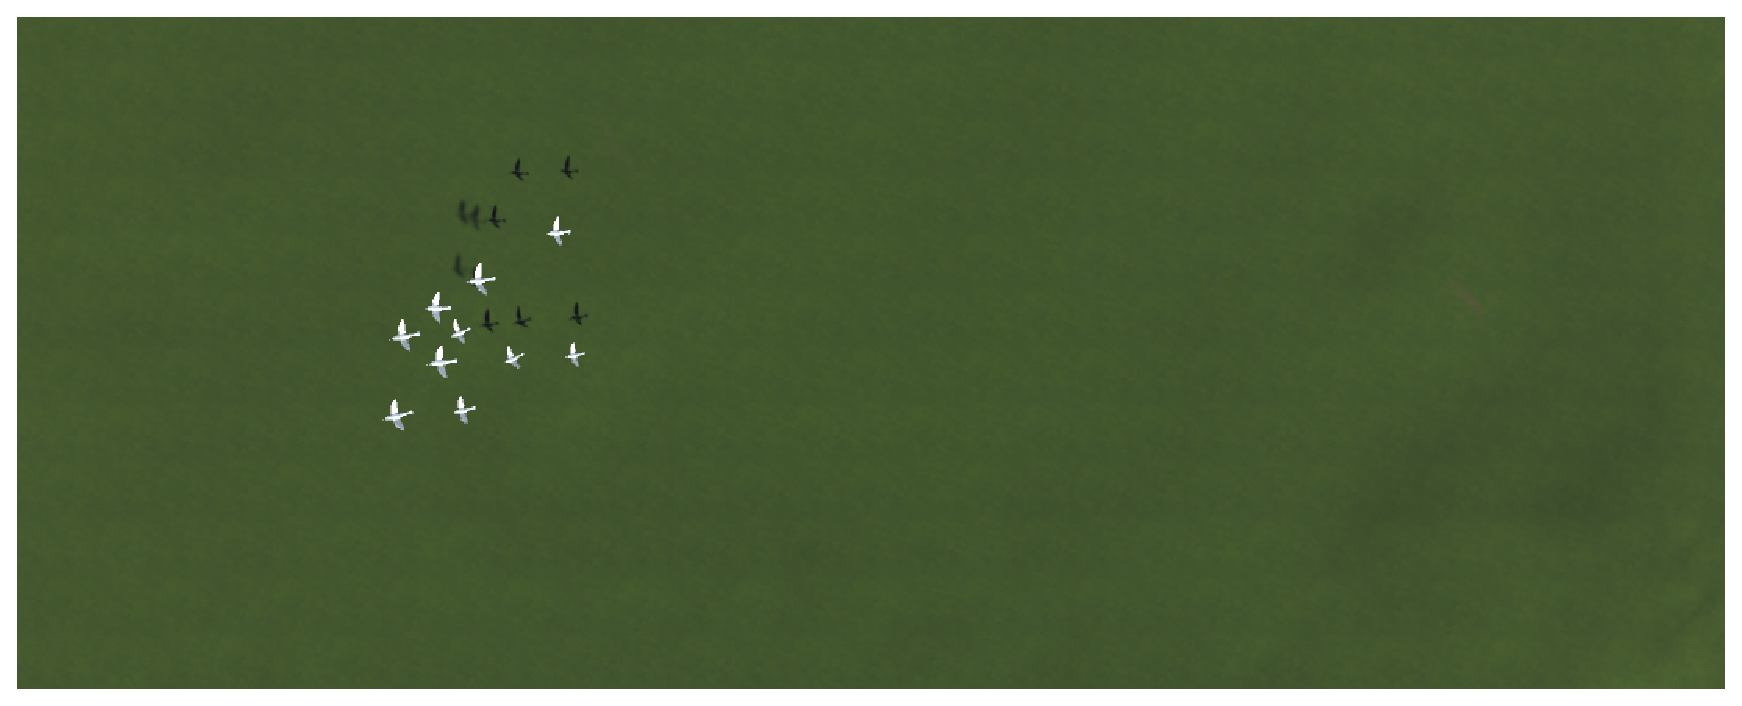
\includegraphics[width=.3\textwidth]{result_2_top_60.eps}}\hspace{\fill}
\subfloat[]{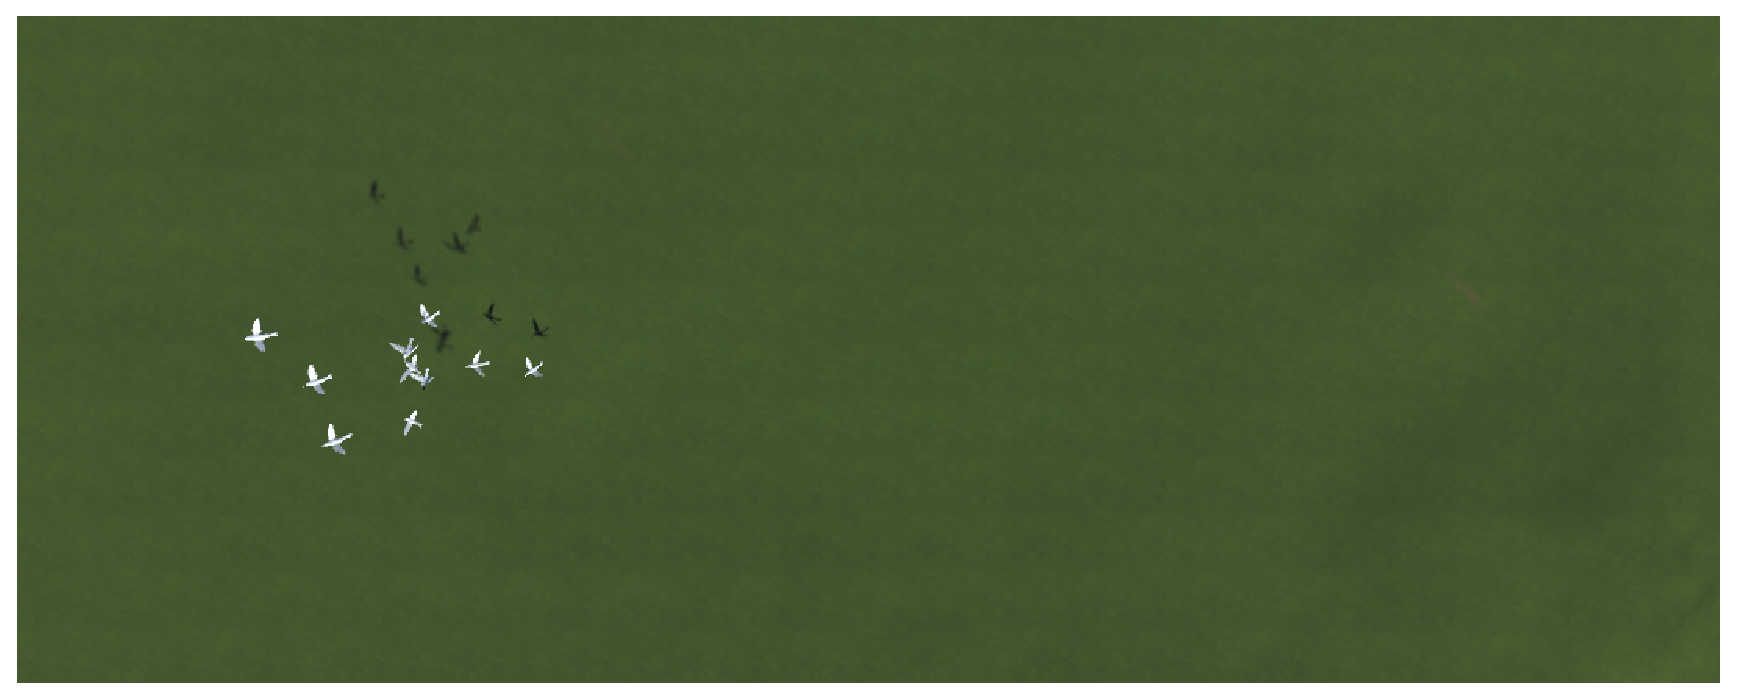
\includegraphics[width=.3\textwidth]{result_2_top_80.eps}}\hspace{\fill}
\subfloat[]{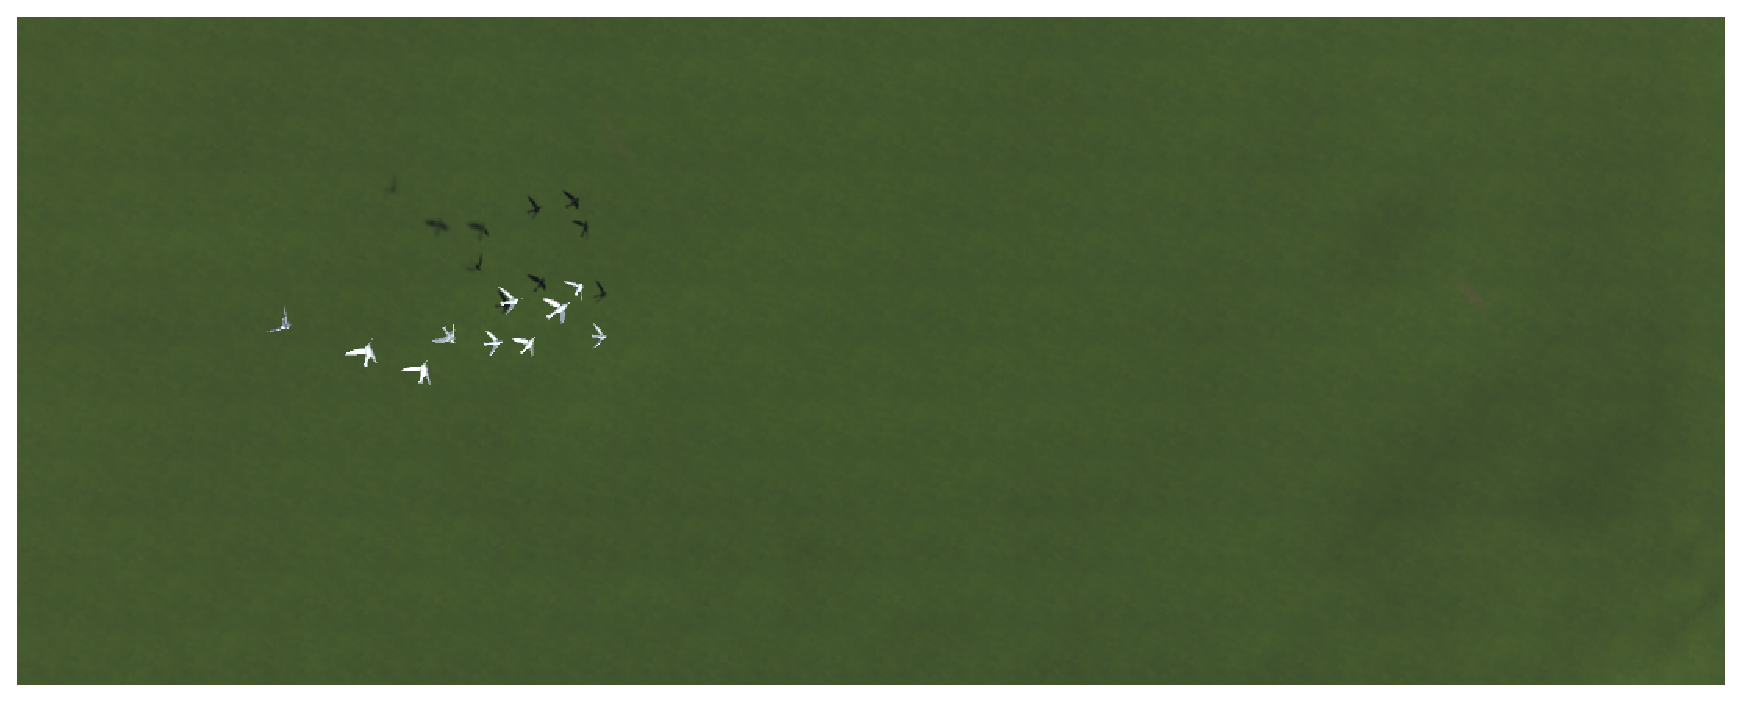
\includegraphics[width=.3\textwidth]{result_2_top_100.eps}}
\end{center}
\caption{Comparison of Result 2 in frame 60, 80, 100.}
\label{figure:result2_com2}
\end{figure}



Figure \ref{figure:result3_com} shows another result from generated video. This time, the birds starts flight in separated position and fly towards each other. in frame ?? and ??, it shows that separation force prevents birds from colliding. This result shows that our system is also capable of generating separated flock motion.